\chapter{暂态：一阶与二阶}\label{ch:b1:transient-regimes}

用力压一下停着的汽车的车角，再松手。
性能良好的汽车弹起一次便停住；
减震器磨损的汽车则要上下晃动
两三次才稳定下来。在电子实验室里，电容器通过线圈放电时，
示波器上也会出现这两种行为：一种是平滑地回归，
另一种是逐渐衰减的振荡。两者都是一个\omterm{def:b1:transient-regimes:firstorder}{稳态}与另一个\omterm{def:b1:transient-regimes:firstorder}{稳态}之间的
\emph{\omterm{def:b1:transient-regimes:firstorder}{暂态}}，且二者都服从同一小类线性微分方程——
只含一个储能元件时为一阶方程，两个储能元件相互交换能量时为二阶方程。
本章一次性求解这些方程，
给出其参数（\omterm{def:b1:transient-regimes:firstorder}{时间常数}、固有频率、\omterm{def:b1:transient-regimes:secondorder}{品质因数}），
并说明同一组数值如何同时描述电路与悬挂系统。

\begin{omfigure}
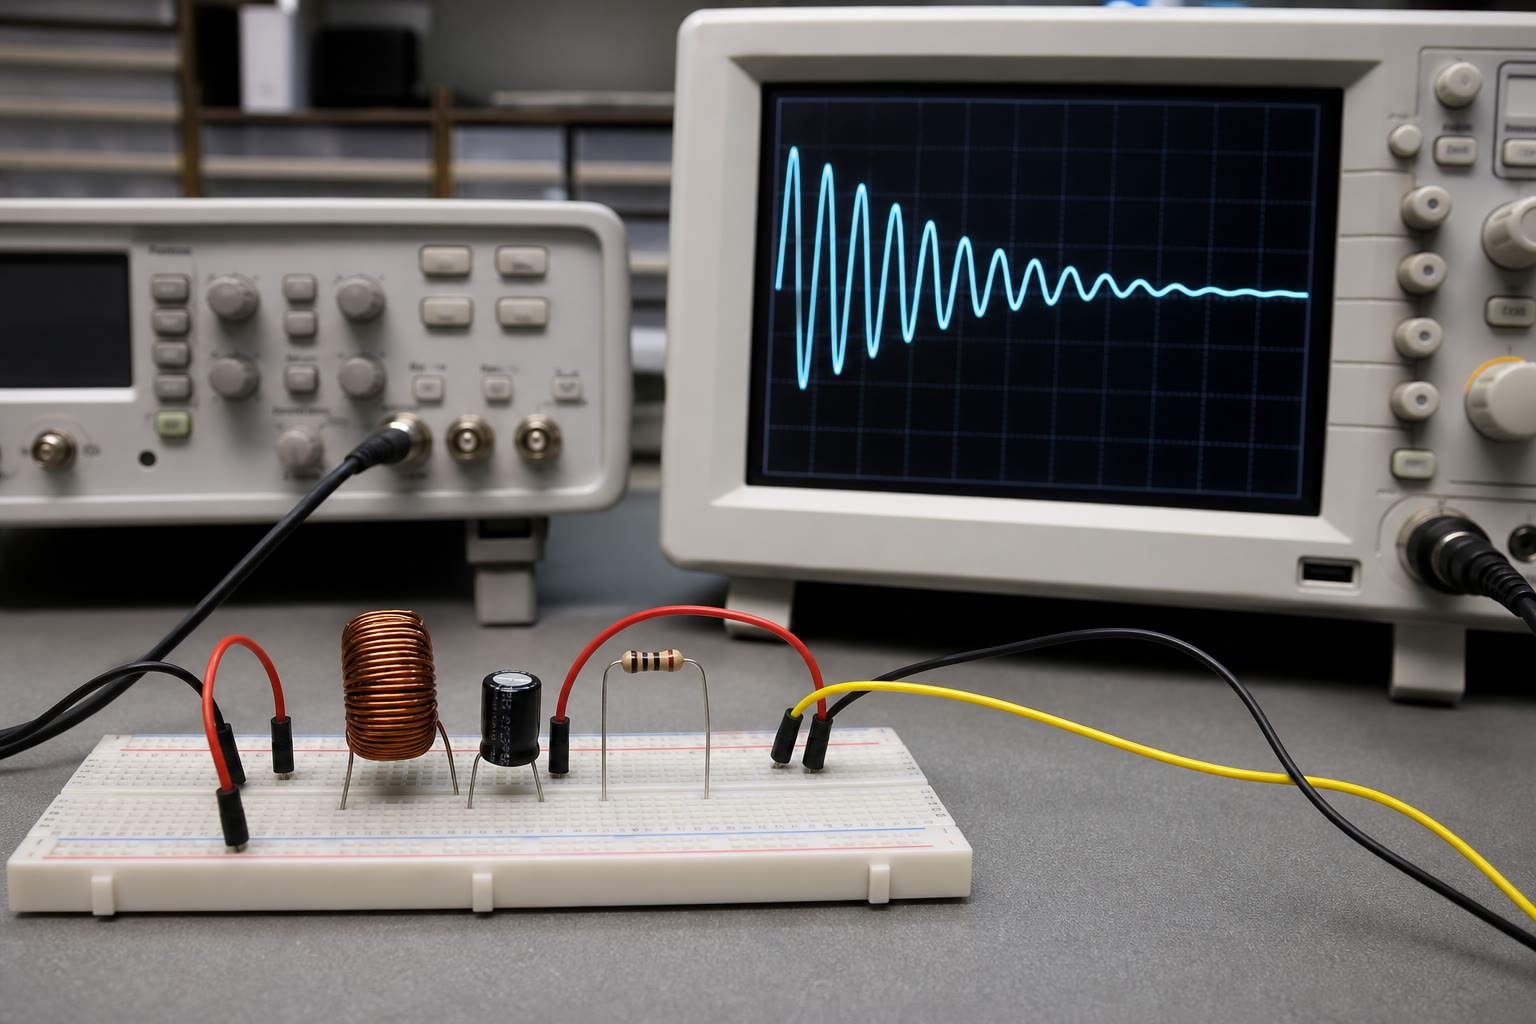
\includegraphics[width=0.60\linewidth]{images/book3/ai/b3-07-rlc-breadboard-oscilloscope.jpg}

{\small 面包板上的线圈、电容器与电阻，以及示波器上阶跃之后出现的衰减振荡：本章讨论的\omterm{thm:b1:transient-regimes:regimes}{准周期}\omterm{def:b1:transient-regimes:firstorder}{暂态}。}
\end{omfigure}

\section{一阶系统}

\begin{definition}[一阶线性系统]\label{def:b1:transient-regimes:firstorder}
\index{一阶系统}\index{时间常数}\index{暂态}\index{稳态}
若某量 $x(t)$ 满足\emph{一阶常系数线性
微分方程}，即
\[
\tau\,\frac{\dd x}{\dd t} + x = x_\infty ,
\]
其中 $\tau > 0$ 为\emph{时间常数}，$x_\infty$ 为常数（
由电源决定的值）。其\emph{稳态}为 $x = x_\infty$；
\emph{暂态}是从初值
$x(0) = x_0$ 出发趋近稳态的过程。
\end{definition}

\begin{theorem}[解]\label{thm:b1:transient-regimes:firstorder}
满足 $x(0) = x_0$ 的唯一解为
\[
x(t) = x_\infty + (x_0 - x_\infty)\,\eu^{-t/\tau} .
\]
与\omterm{def:b1:transient-regimes:firstorder}{稳态}之间的差距，每隔一段时间便缩小为原来的 $\eu^{-1} \approx
0.37$ 倍（间隔为 $\tau$）：$63\%$ 的路程在 $\tau$ 时完成，$95\%$ 在 $3\tau$ 时完成，
$99\%$ 在 $4.6\tau$ 时完成。原点处的切线
到达 $x_\infty$ 的时刻为 $t = \tau$。
\end{theorem}

\begin{proof}
$y = x - x_\infty$ 满足 $\tau y' + y = 0$，其解为
$y = K\eu^{-t/\tau}$（其他解不存在，此结论在线性微分方程的
数学课程中证明）；$K = x_0 - x_\infty$。在 $0$ 处的斜率为
$-(x_0 - x_\infty)/\tau$，若保持此斜率，则经过时间
$\tau$ 即可消除差距。
\end{proof}

\begin{omfigure}
\begin{tikzpicture}
\begin{axis}[omaxis, width=9.4cm, height=5.4cm, xlabel={$t$}, ylabel={$x$},
    xmin=0, xmax=5, ymin=0, ymax=1.35, xtick={1,2,3,4,5},
    xticklabels={$\tau$,$2\tau$,$3\tau$,$4\tau$,$5\tau$},
    ytick={0.632,1}, yticklabels={$0.63$,$x_\infty$}]
  \addplot[omExo, dashed, domain=0:5, samples=2] {1};
  \addplot[omExo, dashed, domain=0:1, samples=2] {x};
  \addplot[omDef, thick, domain=0:5, samples=100] {1 - exp(-x)};
  \draw[dashed, omExo] (axis cs:1,0) -- (axis cs:1,0.632) -- (axis cs:0,0.632);
  \draw[dashed, omExo] (axis cs:3,0) -- (axis cs:3,0.95);
  \node[omExo, below right, font=\footnotesize] at (axis cs:3,0.95) {$0.95\,x_\infty$};
  \node[omDef, font=\footnotesize, below right] at (axis cs:2.2,0.75) {$x_\infty(1 - \eu^{-t/\tau})$};
\end{axis}
\end{tikzpicture}

{\small 从 $x_0 = 0$ 出发的一阶阶跃响应：初始
切线在 $t = \tau$ 处与渐近线相交；$63\%$ 的路程在 $\tau$ 时完成，
$95\%$ 在 $3\tau$ 时完成。每一个一阶\omterm{def:b1:transient-regimes:firstorder}{暂态}都是这条曲线，
沿时间方向按 $\tau$ 拉伸，并按 $x_0$ 与 $x_\infty$ 平移。}
\end{omfigure}

\begin{proposition}[RC 电路与 RL 电路]\label{prop:b1:transient-regimes:rcrl}
\index{RC 电路}\index{RL 电路}
电容器 $C$ 经电阻 $R$ 由理想电源 $E$ 充电时，
满足 $RC\,\dd u_C/\dd t + u_C = E$：$\tau = RC$，$u_{C,\infty} = E$。
线圈 $L$ 与 $R$ 串联后接在 $E$ 两端时，满足 $(L/R)\,\dd i/\dd t + i =
E/R$：$\tau = L/R$，$i_\infty = E/R$。撤去电源（
$E \to 0$）后，同样的方程描述其向零衰减的放电过程。
\end{proposition}

\begin{proof}
由回路定律 $E = Ri + u_C$，其中 $i = C\,\dd u_C/\dd t$；
再由回路定律 $E = Ri + L\,\dd i/\dd t$。
\end{proof}

\begin{proposition}[连续性条件]\label{prop:b1:transient-regimes:continuity}
\index{连续性（$u_C$，$i_L$）}
电容器两端的\omterm{def:b1:dc-circuits:voltage}{电压}与电感器中的电流都是
时间的连续函数：在换接时刻 $t_0$，
有 $u_C(t_0^+) = u_C(t_0^-)$，$i_L(t_0^+) = i_L(t_0^-)$。电阻中的电流与
线圈两端的\omterm{def:b1:dc-circuits:voltage}{电压}可能发生跳变。
\end{proposition}

\begin{proof}
若 $u_C$ 发生跳变，则 $i = C\,\dd u_C/\dd t$ 将为无穷大；
若 $i_L$ 发生跳变，则 $u = L\,\dd i/\dd t$ 将为无穷大。两者在
\omterm{def:b1:dc-circuits:voltage}{电压}与电流有限的电路中均不可能出现（等价地，
储能 $\tfrac12 Cu_C^2$ 与 $\tfrac12 Li^2$ 不可能在瞬间改变，
否则需要无穷大的功率）。
\end{proof}

\begin{method}[求解一阶暂态过程]\label{met:b1:transient-regimes:first}
\begin{enumerate}
  \item 写出开关动作之后的回路定律与节点定律，并代入
        元件关系式；化为关于 $u_C$ 或 $i_L$ 的一个方程，
        并整理成 $\tau x' + x = x_\infty$ 的形式；读出 $\tau$ 与
        $x_\infty$（后者也是将 $C$ 视为断开的电路、$L$ 视为导线时求得的
        \omterm{def:b1:transient-regimes:firstorder}{稳态}）。
  \item 求 $x_0$：利用换接时刻 $u_C$ 或 $i_L$ 的连续性，
        应使用换接\emph{之前}的电路。
  \item 写出 $x = x_\infty + (x_0 - x_\infty)\eu^{-t/\tau}$；再
        通过求导及回路定律求出其他量。
\end{enumerate}
当电容器两端所接为由电阻与电源组成的网络时，先将该网络替换为
其戴维南等效电路 $(E_{\mathrm{Th}}, R_{\mathrm{Th}})$（见
\cref{ch:b1:dc-circuits}）：$\tau = R_{\mathrm{Th}}C$，
$u_\infty = E_{\mathrm{Th}}$。
\end{method}

\begin{proposition}[RC 充电的能量平衡]\label{prop:b1:transient-regimes:rcenergy}
将电容器从 $0$ 充至 $E$（经任意电阻 $R$）时，
电源提供 $CE^2$，电容器储存 $\tfrac12 CE^2$，
而电阻耗散另外的 $\tfrac12 CE^2$——无论 $R$ 取何值。
\end{proposition}

\begin{proof}
$i = (E/R)\eu^{-t/\tau}$；电源提供的能量为 $\int_0^\infty Ei\,\dd t
= E \cdot (E/R)\tau = CE^2$；电阻吸收的能量为 $\int_0^\infty Ri^2\,\dd t
= (E^2/R)\int_0^\infty \eu^{-2t/\tau}\dd t = (E^2/R)(\tau/2) = \tfrac12 CE^2$；
两者之差即为所储存的 $\tfrac12 CE^2$。较小的 $R$ 会更快地
耗散同样的能量。
\end{proof}

\begin{example}[继电器线圈]\label{ex:b1:transient-regimes:relay}
$L = \qty{20}{mH}$，$R = \qty{5.0}{\ohm}$，$E = \qty{10}{V}$：$\tau =
\qty{4.0}{ms}$，$i_\infty = \qty{2.0}{A}$；触点在
$i$ 达到 \qty{1.5}{A} 时吸合，即于 $t = -\tau\ln(1 - 0.75) =
\qty{5.5}{ms}$ 时刻。断开电路时，$i$ 须自 \qty{2}{A} 开始下降；
在线圈两端并联一只“续流”二极管，使电流仅经 $R$
形成通路，$\tau = \qty{4}{ms}$，而非产生电火花。
\end{example}

\section{二阶系统}

\begin{definition}[二阶系统的标准形式]\label{def:b1:transient-regimes:secondorder}
\index{二阶线性系统}\index{固有角频率}\index{品质因数}\index{阻尼比}
若\omterm{def:b1:units-dimensions:unit}{物理量} $x(t)$ 满足下式，则称其为\emph{二阶线性系统}：
\[
\frac{\dd^2 x}{\dd t^2} + \frac{\omega_0}{Q}\,\frac{\dd x}{\dd t} + \omega_0^2\,x
= \omega_0^2\,x_\infty ,
\]
其中 $\omega_0 > 0$ 为\emph{固有\omterm{def:b1:wave-propagation:signal}{角频率}}，$Q > 0$ 为
\emph{品质因数}（无量纲），$x_\infty$ 为\omterm{def:b1:transient-regimes:firstorder}{稳态}。
亦可记为 $\omega_0/Q = 2\xi\omega_0$，其中 $\xi = 1/2Q$ 为
\emph{阻尼比}。
\end{definition}

\begin{proposition}[串联 RLC 电路]\label{prop:b1:transient-regimes:rlc}
\index{RLC 电路}
电容器 $C$、线圈 $L$ 与电阻 $R$ 串联，并接于
电源 $E$ 两端时，电容器\omterm{def:b1:dc-circuits:voltage}{电压}服从标准形式，其参数为
\[
\omega_0 = \frac{1}{\sqrt{LC}}, \qquad Q = \frac{1}{R}\sqrt{\frac{L}{C}},
\qquad u_{C,\infty} = E .
\]
\end{proposition}

\begin{proof}
由回路定律 $E = L\,\dd i/\dd t + Ri + u_C$，代入 $i = C\,\dd u_C/\dd t$：
$LC\,u_C'' + RC\,u_C' + u_C = E$；两边除以 $LC$，可得
$\omega_0^2 = 1/LC$，$\omega_0/Q = R/L$。
\end{proof}

\begin{omfigure}
\begin{tikzpicture}[font=\small]
  \draw (0,0) to[battery1, l=$E$, invert] (0,2.6) to[R=$R$] (2.4,2.6) to[L=$L$, i=$i$] (4.8,2.6) -- (4.8,2.6) to[C=$C$, v=$u_C$] (4.8,0) -- (0,0);
  \begin{scope}[xshift=7.6cm]
    \draw[thick] (0,0) -- (0,3.4);
    \fill[pattern=north east lines] (-0.25,0) rectangle (0,3.4);
    % spring
    \draw[thick] (0,2.6) -- (0.4,2.6) \foreach \i in {0,...,5} {-- ++(0.2,0.25) -- ++(0.2,-0.5) -- ++(0.2,0.25)} -- (3.3,2.6);
    % damper
    \draw[thick] (0,0.8) -- (1.2,0.8);
    \draw[thick] (1.2,0.5) -- (1.2,1.1) -- (2.2,1.1); \draw[thick] (1.2,0.5) -- (2.2,0.5);
    \draw[thick] (1.9,0.6) -- (1.9,1.0); \draw[thick] (1.9,0.8) -- (3.3,0.8);
    \draw[thick, fill=omDef!15] (3.3,0.2) rectangle (4.5,3.2); \node at (3.9,1.7) {$m$};
    \draw[-Stealth] (3.9,3.5) -- (5.2,3.5) node[right] {$x$};
    \node at (1.7,3.15) {$k$}; \node at (1.7,0.1) {$\alpha$};
  \end{scope}
\end{tikzpicture}

{\small 二阶系统的两种实例：串联 \omterm{prop:b1:transient-regimes:rlc}{RLC
电路}（$\omega_0 = 1/\sqrt{LC}$，$Q = \sqrt{L/C}/R$）与
\omterm{prop:b1:transient-regimes:mechanical}{质量–弹簧–阻尼器}（$\omega_0 = \sqrt{k/m}$，$Q = \sqrt{km}/\alpha$）。
方程相同，三种情形亦相同。}
\end{omfigure}

\begin{proposition}[机械振子]\label{prop:b1:transient-regimes:mechanical}
\index{质量–弹簧–阻尼器}\index{机电类比}
质量为 $m$ 的物体系于劲度系数为 $k$ 的弹簧上，并连有黏滞阻尼器，
阻尼系数为 $\alpha$（阻尼力为 $-\alpha\dot x$），物体偏离平衡位置的位移为 $x$，
满足 $m\ddot x + \alpha\dot x + kx = 0$，属于标准形式，
参数为：
\[
\omega_0 = \sqrt{\frac{k}{m}}, \qquad Q = \frac{\sqrt{km}}{\alpha} .
\]
对应关系为 $x \leftrightarrow q$，$\dot x \leftrightarrow i$，
$m \leftrightarrow L$，$\alpha \leftrightarrow R$，$k \leftrightarrow 1/C$
使一个系统的每一结论都映射到另一个系统上。
\end{proposition}

\begin{proof}
由牛顿第二定律（见\cref{ch:b1:newton-dynamics}），
代入弹簧力 $-kx$ 与阻尼力，两边除以 $m$。
\end{proof}

\begin{theorem}[三种情形]\label{thm:b1:transient-regimes:regimes}
\index{非周期情形}\index{临界情形}\index{准周期情形}\index{准周期}
齐次方程 $x'' + (\omega_0/Q)x' +
\omega_0^2 x = 0$ 的解由 $r^2 + (\omega_0/Q)r +
\omega_0^2 = 0$ 的根决定，其判别式为 $\Delta = \omega_0^2(1/Q^2 - 4)$：
\begin{itemize}
  \item 当 $Q < \tfrac12$ 时，\emph{\omterm{thm:b1:transient-regimes:regimes}{非周期情形}}：两个负实根
        $r_\pm = -\frac{\omega_0}{2Q}\big(1 \mp \sqrt{1 - 4Q^2}\big)$，
        $x = A\eu^{r_+t} + B\eu^{r_-t}$，无振荡地回归；
  \item 当 $Q = \tfrac12$ 时，\emph{\omterm{thm:b1:transient-regimes:regimes}{临界情形}}：二重根 $r = -\omega_0$，
        $x = (A + Bt)\eu^{-\omega_0 t}$，回归最快，
        且无超调；
  \item 当 $Q > \tfrac12$ 时，\emph{\omterm{thm:b1:transient-regimes:regimes}{准周期情形}}：复根
        $r = -1/\tau \pm \iu\omega$，其中
        \[
        \tau = \frac{2Q}{\omega_0}, \qquad
        \omega = \omega_0\sqrt{1 - \frac{1}{4Q^2}},
        \qquad
        x = \eu^{-t/\tau}\big(A\cos\omega t + B\sin\omega t\big),
        \]
        即阻尼振荡，其\emph{\omterm{thm:b1:transient-regimes:regimes}{准周期}}为 $T = 2\pi/\omega$，
        振荡位于包络 $\pm\sqrt{A^2 + B^2}\,\eu^{-t/\tau}$ 之内。
\end{itemize}
右端为常数时，完整解为 $x_\infty$ 与
齐次方程的解之和；$A$、$B$ 由 $x(0)$ 和 $x'(0)$ 确定。
\end{theorem}

\begin{proof}
常系数线性方程的特征方程（数学课程中的二阶线性方程）：
其根为
$r = -\omega_0/2Q \pm \tfrac12\sqrt\Delta$。当 $Q > \tfrac12$ 时，
$\sqrt\Delta = \iu\omega_0\sqrt{4 - 1/Q^2}$，于是实部为
$-\omega_0/2Q = -1/\tau$，虚部为 $\pm\omega_0\sqrt{1 - 1/4Q^2}$；
实解即 $\eu^{-t/\tau}\cos\omega t$ 与
$\eu^{-t/\tau}\sin\omega t$ 的线性组合。
\end{proof}

\begin{omfigure}
\begin{tikzpicture}
\begin{axis}[omaxis, width=11.5cm, height=6cm, xlabel={$\omega_0 t$}, ylabel={$x/x_\infty$},
    xmin=0, xmax=16, ymin=0, ymax=1.75, xtick={0,5,10,15}, ytick={0.5,1,1.5},
    legend style={at={(0.97,0.97)}, anchor=north east, font=\footnotesize, draw=none, fill=none}]
  % Q=0.2: roots r = -(1/(2Q))(1 -/+ sqrt(1-4Q^2)) = -2.5(1 -/+ 0.6) = -1, -4 ; x = 1 - (4 e^{-t} - e^{-4t})/3
  \addplot[omProp, thick, domain=0:16, samples=200] {1 - (4*exp(-x) - exp(-4*x))/3};
  \addlegendentry{$Q = 0.2$（非周期的）}
  \addplot[omThm, thick, domain=0:16, samples=200] {1 - (1 + x)*exp(-x)};
  \addlegendentry{$Q = 0.5$（临界）}
  % Q=3: tau=6, w = sqrt(1-1/36)=0.986 ; x = 1 - e^{-t/6}(cos wt + sin wt /(6 w))
  \addplot[omDef, thick, domain=0:16, samples=400] {1 - exp(-x/6)*(cos(deg(0.986*x)) + sin(deg(0.986*x))/(6*0.986))};
  \addlegendentry{$Q = 3$（准周期的）}
  \addplot[omExo, dashed, domain=0:16, samples=2] {1};
\end{axis}
\end{tikzpicture}

{\small 二阶系统从静止出发的阶跃响应，对三个不同的
\omterm{def:b1:transient-regimes:secondorder}{品质因数}：$Q$ 较小时为缓慢爬升；$Q = \tfrac12$ 时为无超调的最快回归；
$Q$ 较大时出现振铃，持续约 $Q$ 次
振荡。}
\end{omfigure}

\begin{proposition}[由准周期曲线读出 $Q$]\label{prop:b1:transient-regimes:decrement}
\index{对数衰减率}
在\omterm{thm:b1:transient-regimes:regimes}{准周期情形}下，相邻两个极大值之比为
$x_{n+1}/x_n = \eu^{-T/\tau}$；\emph{\omterm{prop:b1:transient-regimes:decrement}{对数衰减率}}定义为
\[
\delta = \ln\frac{x_n}{x_{n+1}} = \frac{T}{\tau} = \frac{\pi}{Q\sqrt{1 - 1/4Q^2}}
\approx \frac{\pi}{Q} \quad (Q \gg 1)
\]
由此给出 $Q$；可见振荡的次数，
即\omterm{def:b1:wave-propagation:signal}{振幅}降至 $5\%$ 以下之前，约为 $Q$。当 $Q \gg 1$ 时，$\omega \approx \omega_0$
且 $T \approx 2\pi/\omega_0$。
\end{proposition}

\begin{proof}
包络 $\eu^{-t/\tau}$ 每周期乘以 $\eu^{-T/\tau}$；
$T/\tau = (2\pi/\omega)(\omega_0/2Q)$。包络在 $\eu^{-3}
\approx 5\%$ 时，即 $3\tau = 6Q/\omega_0 \approx Q\,T$，
约经过 $Q$ 个周期。
\end{proof}

\begin{omfigure}
\begin{tikzpicture}
\begin{axis}[omaxis, width=11.5cm, height=5.6cm, xlabel={$t$}, ylabel={$x$},
    xmin=0, xmax=12.5, ymin=-1.2, ymax=1.3, xtick={2,4,6,8,10,12},
    xticklabels={$T$,$2T$,$3T$,$4T$,$5T$,$6T$}, ytick={-1,1}, yticklabels={$-x_0$,$x_0$}]
  \addplot[omExo, dashed, domain=0:12.5, samples=60] {exp(-x/5)};
  \addplot[omExo, dashed, domain=0:12.5, samples=60] {-exp(-x/5)};
  \addplot[omDef, thick, domain=0:12.5, samples=500] {exp(-x/5)*cos(deg(pi*x))};
  \fill[omThm] (axis cs:0,1) circle (1.4pt) node[above right, font=\footnotesize] {$x_0$};
  \fill[omThm] (axis cs:2,0.670) circle (1.4pt) node[above right, xshift=2pt, yshift=3pt, font=\footnotesize] {$x_1 = x_0\eu^{-T/\tau}$};
  \fill[omThm] (axis cs:4,0.449) circle (1.4pt) node[above right, xshift=2pt, yshift=3pt, font=\footnotesize] {$x_2$};
\end{axis}
\end{tikzpicture}

{\small 自由\omterm{thm:b1:transient-regimes:regimes}{准周期}衰减，$x = x_0\eu^{-t/\tau}\cos\omega t$：
相邻极大值按固定因子 $\eu^{-T/\tau}$ 减小，且
$\ln(x_n/x_{n+1}) = T/\tau \approx \pi/Q$ 给出\omterm{def:b1:transient-regimes:secondorder}{品质因数}，
可由曲线读出。}
\end{omfigure}

\begin{example}[RLC 电路的振铃]\label{ex:b1:transient-regimes:rlcnum}
$L = \qty{10}{mH}$, $C = \qty{100}{nF}$, $R = \qty{100}{\ohm}$:
$\omega_0 = 1/\sqrt{10^{-9}} = \qty{3.16e4}{rad/s}$ ($f_0 =
\qty{5.03}{kHz}$），$Q = \sqrt{L/C}/R = 316/100 = 3.16$：\omterm{thm:b1:transient-regimes:regimes}{准周期情形}，
$\tau = 2Q/\omega_0 = \qty{0.20}{ms}$, $\omega = 0.987\,\omega_0$,
$T = \qty{0.20}{ms}$，可见三次振荡。临界电阻
为 $R_c = 2\sqrt{L/C} = \qty{632}{\ohm}$，超过此值时放电
为非周期的。
\end{example}

\begin{method}[二阶暂态的求解]\label{met:b1:transient-regimes:second}
\begin{enumerate}
  \item 写出方程；化为标准形式；读出 $\omega_0$，
        $Q$ 与 $x_\infty$。
  \item 由 $Q$ 判定情形，并将通解写成
        $x_\infty$ 与齐次方程的解之和。
  \item 求 $x(0)$ 和 $x'(0)$，依据 $u_C$ 与 $i_L$ 的连续性；
        （对 RLC 电路：$u_C(0^+) = u_C(0^-)$ 且 $u_C'(0^+) = i(0^-)/C$）；
        解出两个常数。
\end{enumerate}
\end{method}

\begin{example}[初始条件]\label{ex:b1:transient-regimes:ic}
上例中的电容器充电至 $U_0$，并于
$t = 0$ 时闭合开关，接到 $L$ 与 $R$ 上（无电源）：$x_\infty = 0$，
$u_C(0) = U_0$，$u_C'(0) = i(0)/C = 0$，因线圈中原无电流。
由此得 $A = U_0$，且 $-A/\tau + B\omega = 0$，$B = U_0/(\omega\tau) =
U_0/\sqrt{4Q^2 - 1}$，于是 $u_C = U_0\eu^{-t/\tau}[\cos\omega t + \sin(\omega
t)/\sqrt{4Q^2 - 1}]$——当 $Q \gg 1$ 时简化为 $U_0\eu^{-t/\tau}\cos\omega_0 t$，
而电流 $i = -C\,\dd u_C/\dd t$ 的峰值约在 $U_0\sqrt{C/L} =
U_0/(\omega_0 L)$ 附近。
\end{example}

\begin{remark}[能量]\label{rem:b1:transient-regimes:energy}
储存能量 $\tfrac12 Cu_C^2 + \tfrac12 Li^2$（或 $\tfrac12 kx^2
+ \tfrac12 m\dot x^2$）以速率 $Ri^2$（$\alpha\dot x^2$）减少：
对其求导并利用方程。每经过一个\omterm{thm:b1:transient-regimes:regimes}{准周期}，能量
减为原来的 $\eu^{-2T/\tau}$ 倍；当 $Q = 3$ 时，每次振荡约
损失其中的 $88\%$。$Q$ 大意味着相对于振荡而言能量泄漏缓慢——
是好的计时器，也是尖锐的共振
（见\cref{ch:b1:sinusoidal-impedance}）——而 $Q$ 小则回复迅速：
宜用于悬挂装置或仪表指针。
\end{remark}

\section{练习}

\begin{exercise}[$\star$]\label{exo:b1:transient-regimes:1}
一个 RC 电路：$R = \qty{10}{k\ohm}$，$C = \qty{47}{nF}$，由 $E$ 充电。
求 $\tau$、$u_C(\tau)/E$，以及达到 $99\%$ 的 $E$ 所需的时间。
\end{exercise}

\begin{exercise}[$\star$]\label{exo:b1:transient-regimes:2}
一个 RL 电路：$L = \qty{20}{mH}$，$R = \qty{5.0}{\ohm}$，$E = \qty{10}{V}$。
求 $\tau$、最终电流、$t = \tau$ 时的电流，以及
合上开关后瞬间线圈两端的\omterm{def:b1:dc-circuits:voltage}{电压}。
\end{exercise}

\begin{exercise}[$\star$]\label{exo:b1:transient-regimes:3}
一个串联 RLC 电路：$L = \qty{10}{mH}$，$C = \qty{100}{nF}$，$R = \qty{100}{\ohm}$。
求 $\omega_0$、$f_0$、$Q$；说明其所属的状态，并给出
$\tau$ 以及\omterm{thm:b1:transient-regimes:regimes}{准周期}。
\end{exercise}

\begin{exercise}[$\star$]\label{exo:b1:transient-regimes:4}
对于相同的 $L$ 和 $C$，多大的电阻使电路处于临界状态？
此时 $Q$ 为多少？若 $R = \qty{2}{k\ohm}$，会发生什么？
\end{exercise}

\begin{exercise}[$\star\star$]\label{exo:b1:transient-regimes:5}
一个带电电容器 $C = \qty{1.0}{\micro F}$ 通过
未知电阻 $R$ 放电，\omterm{def:b1:dc-circuits:voltage}{电压}每经过 \qty{3.5}{ms} 减半。证明
半衰期为 $\tau\ln 2$，并求 $R$。
\end{exercise}

\begin{exercise}[$\star\star$]\label{exo:b1:transient-regimes:6}
用直接积分证明：电容器从 $0$ 充电至 $E$
的过程中，经 $R$ 恰好耗散 $\tfrac12 CE^2$ 于 $R$ 上，与
$R$ 无关。传输效率会怎样，
又怎样才能做得更好？
\end{exercise}

\begin{exercise}[$\star\star$]\label{exo:b1:transient-regimes:7}
在示波器上，自由 RLC 衰减的连续极大值依次为
\qty{2.0}{V}、\qty{1.5}{V}、\qty{1.12}{V}，
相邻极大值的时间间隔为 \qty{0.40}{ms}。推出 $Q$、$\omega_0$，并在 $C = \qty{1.0}{\micro F}$ 的条件下求
$L$ 和 $R$ 的值。
\end{exercise}

\begin{exercise}[$\star\star$]\label{exo:b1:transient-regimes:8}
电容器充电至 $U_0 = \qty{100}{V}$（$C = \qty{10}{\micro F}$）后，
切换到电阻很小的线圈 $L = \qty{1.0}{mH}$ 上（$Q \gg 1$）。
写出 $u_C(t)$ 与 $i(t)$，并估算峰值电流。在峰值处，
能量位于何处？
\end{exercise}

\begin{exercise}[$\star\star$]\label{exo:b1:transient-regimes:9}
汽车的四分之一模型：$m = \qty{400}{kg}$ 的质量块置于弹簧 $k = \qty{2.0e4}{N/m}$ 上。
求 $\omega_0$、$f_0$ 以及临界阻尼系数。若
减振器 $\alpha = \qty{2000}{N.s/m}$，求 $Q$、所属状态、
\omterm{thm:b1:transient-regimes:regimes}{准周期}以及衰减时间 $\tau$。
\end{exercise}

\begin{exercise}[$\star\star\star$]\label{exo:b1:transient-regimes:10}
线圈 $L = \qty{0.50}{H}$ 中通有电流 $I_0 = \qty{2.0}{A}$；电源断开后，
线圈仅与泄放电阻 $R = \qty{100}{\ohm}$ 相接。
求 $i(t)$、$\tau$、线圈两端的峰值\omterm{def:b1:dc-circuits:voltage}{电压}以及
耗散的能量。若没有该电阻，会发生什么？
\end{exercise}

\begin{exercise}[$\star\star\star$]\label{exo:b1:transient-regimes:11}
电容器 $C = \qty{1.0}{\micro F}$ 由 $E = \qty{12}{V}$ 经
$R_1 = \qty{10}{k\ohm}$ 充电，同时 $R_2 = \qty{20}{k\ohm}$
并联在其两端。利用戴维南等效，求\omterm{def:b1:transient-regimes:firstorder}{时间常数}以及
最终\omterm{def:b1:dc-circuits:voltage}{电压}；写出 $u_C(t)$（$u_C(0) = 0$）。
\end{exercise}

\begin{exercise}[$\star\star\star$]\label{exo:b1:transient-regimes:12}
临界状态，从静止开始的阶跃（$x(0) = x'(0) = 0$）：证明
$x = x_\infty[1 - (1 + \omega_0 t)\eu^{-\omega_0 t}]$，并
数值求出达到 $95\%$ 的 $x_\infty$ 所需的时间（以
$1/\omega_0$ 为单位）。与 $Q = 5$ 时包络的稳定时间相比，
并与 $Q = 0.1$ 时慢根的情形相比较，由此说明为何“临界”
是工程师的目标。
\end{exercise}

\section{问题：设计悬挂系统}

\begin{problem}[{周末问题——同一微分方程在实验台上与汽车底盘下：
一个磨损的减振器允许多少次弹跳，设计者转而选择什么，
以及如何用一个数判别两者，
并把它们区分开}]
\label{pb:b1:transient-regimes:1}
第一部分研究串联 RLC 电路，$L = \qty{10}{mH}$，$C = \qty{100}{nF}$；
第二至第四部分研究四分之一车模型：质量 $m = \qty{350}{kg}$ 的物块置于
弹簧 $k = \qty{22}{kN/m}$ 上，减振器施加 $-\alpha\dot x$。
\omterm{thm:b1:transient-regimes:regimes}{准周期}区域中阶跃响应的过冲（已给出）：
$x_{\max}/x_\infty - 1 = \exp(-\pi\xi/\sqrt{1 - \xi^2})$, $\xi = 1/2Q$.

\medskip
\noindent\textbf{第一部分——电路。}
\begin{enumerate}
  \item 写出串联 RLC 接于电源 $E$ 两端的回路方程，以及
        $u_C$ 满足的微分方程。
  \item 将其化为标准形式，并表示出 $\omega_0$ 与 $Q$。
  \item 求 $\omega_0$、$f_0$ 以及临界电阻 $R_c$。
  \item 写出特征方程及其判别式；
        用 $Q$ 叙述三种状态。
  \item 在\omterm{thm:b1:transient-regimes:regimes}{准周期情形}下，给出 $\tau$ 与 $\omega$ 以及
        $u_C(t)$ 的形式。
  \item 当 $R = \qty{100}{\ohm}$ 时，求 $Q$、$\tau$、\omterm{thm:b1:transient-regimes:regimes}{准周期}，
        以及可见振荡的次数。
  \item 电容器充电至 $U_0$ 后切换到 $L$ 与 $R$ 上，
        于 $t = 0$ 时给出 $u_C(0^+)$ 与 $\dd u_C/\dd t(0^+)$，
        并说明各自的物理原因。
\end{enumerate}

\medskip
\noindent\textbf{第二部分——四分之一车}
\begin{enumerate}[resume]
  \item 以平衡位置为起点度量 $x$，写出物体的牛顿
        第二定律，并证明重力项消去。
  \item 将方程化为标准形式，求 $\omega_0$ 与 $Q$（以 $m$、$k$、$\alpha$ 表示），
        并列出机电
        对应关系。
  \item 求 $\omega_0$、$f_0$ 以及临界阻尼系数
        $\alpha_c$。
  \item 设计者取 $\alpha = \qty{4000}{N.s/m}$，求 $Q$、
        $\xi$，并指出所属状态。
  \item 求 $\tau$ 与\omterm{thm:b1:transient-regimes:regimes}{准周期}。
  \item 求经过阶跃输入（路沿）后的超调量：
        车是否舒适？
  \item 第一部分的电路需取多大的电阻 $R$，
        才能使其 $Q$ 与本悬挂相同？
\end{enumerate}

\medskip
\noindent\textbf{第三部分——磨损的阻尼器}
油液已泄漏：$\alpha = \qty{1200}{N.s/m}$。
\begin{enumerate}[resume]
  \item 求 $Q$、\omterm{thm:b1:transient-regimes:regimes}{准周期}与 $\tau$。
  \item 相邻极大值按何倍数减小？在\omterm{def:b1:wave-propagation:signal}{振幅}降至 $5\%$ 以下前，
        还能看到几次弹跳？
  \item 弹跳试验：将车角向下压 $x_0 =
        \qty{5.0}{cm}$ 后释放，给出初始条件、
        弹簧中储存的能量，并说明该能量去向何处。
  \item 估算首次回到平衡位置时物体的最大速度
        （$\approx x_0\omega_0$，$Q \gg 1$ 时）以及阻尼器的
        最大阻尼力。
  \item 为何恰好临界阻尼（$Q = \tfrac12$）并非设计者的选择，
        尽管它没有超调？（想一想
        回程最后几毫米。）
  \item 求磨损阻尼器的超调量，并与
        第二部分比较。
\end{enumerate}

\medskip
\noindent\textbf{第四部分——由记录曲线诊断 $Q$}
车身上的加速度计记录了自由衰减过程。
\begin{enumerate}[resume]
  \item 对磨损车，相邻极大值依次为 $1.00$、$0.25$、$0.062$
        （任意单位）。求\omterm{prop:b1:transient-regimes:decrement}{对数衰减率}，
        精确求出 $\xi$（由 $\delta = 2\pi\xi/\sqrt{1 - \xi^2}$），再求 $Q$；
        与第三部分比较。
  \item 对完好的车，看不到第二个极大值；只能读出
        超调量 $3.8\%$。由超调公式反解
        求 $\xi$ 与 $Q$。
  \item 磨损阻尼器每个\omterm{thm:b1:transient-regimes:regimes}{准周期}耗散的机械能
        占其机械能的比例是多少？
  \item 若手边没有车，技术人员按第一部分搭建 RLC 电路，
        取 $R$ 使 $Q = 2.3$，应取多大的 $R$，并说明为何
        以 $\omega_0 t$ 为横坐标绘制的示波器波形
        与车的波形形状完全相同？
  \item 总结：何种无量纲数决定任一二阶\omterm{def:b1:transient-regimes:firstorder}{暂态}的形状，
        悬挂设计者应追求的取值为何，
        以及驾驶者从“不止
        一次弹跳”应得出什么结论。
\end{enumerate}
\end{problem}
